% NeurIPS 2026 submission template (uses 2024 style; swap to neurips_2026.sty when released).
\documentclass{article}

\usepackage[final]{neurips_2025}
\usepackage[utf8]{inputenc}
\usepackage[T1]{fontenc}
\usepackage{hyperref}
\usepackage{url}
\usepackage{booktabs}
\usepackage{amsfonts}
\usepackage{amsmath}
\usepackage{amssymb}
\usepackage{amsthm}
\usepackage{microtype}
\usepackage{graphicx}
\usepackage{xcolor}

\newtheorem{theorem}{Theorem}
\newtheorem{proposition}[theorem]{Proposition}
\newtheorem{lemma}[theorem]{Lemma}
\theoremstyle{definition}
\newtheorem{assumption}{Assumption}
\theoremstyle{remark}
\newtheorem{remark}{Remark}

\DeclareMathOperator{\E}{\mathbb{E}}
\DeclareMathOperator{\Prob}{\mathbb{P}}
\DeclareMathOperator{\Ind}{\mathbb{I}}
\newcommand{\R}{\mathbb{R}}
\newcommand{\sphere}{\mathcal{S}^{d-1}}
\newcommand{\vmf}{\mathrm{vMF}}
\newcommand{\Ad}{A_d}

\title{Compound E-Values for FDR-Controlled Coordination Detection \\
in Regulatory Public-Comment Dockets}

\author{Anonymous Authors\\
Anonymous Affiliations\\
\texttt{anonymous@anonymous.org}
}

\begin{document}

\maketitle

\begin{abstract}
Twenty-two million public comments arrived at the FCC during a single 2017 net-neutrality proceeding, and a 2021 government investigation later attributed the majority to paid contractors who paraphrased master templates to fabricate submissions on behalf of broadband-industry clients, yet the coordination-detection tools available to regulators and researchers remain built for the verbatim form-letter campaigns of an earlier era. The natural test statistics on the sphere of normalized text embeddings --- mean cohesion, vMF concentration, likelihood under a fitted vMF template --- are in fact anti-correlated with paid-astroturf attribution on real corpora, because paid contractors paraphrase to evade near-duplicate detection while grassroots advocacy organizations copy templates verbatim. We develop a five-stage framework that borrows the architecture of compound e-values from multiple-testing theory and applies it to cluster-level coordination detection, treating each candidate cluster as jointly determined by systematic corpus-marginal density and idiosyncratic template structure. The framework embeds raw comments to a high-dimensional sphere via a sentence-transformer, extracts candidate clusters through Leiden community detection at coarse resolution, computes a multi-resolution fragmentation rate that distinguishes verbatim coordination (low fragmentation) from paraphrase coordination (high fragmentation), calibrates a verbatim-versus-paraphrase likelihood ratio through unsupervised Beta-mixture EM with no labels, and aggregates per-cluster e-values through the e-BH procedure to control false discovery rate at level $\alpha$ under arbitrary dependence between clusters. Validated against 6{,}072 paid-astroturf clusters identified by the 2021 New York Attorney General investigation across 15{,}748 candidate clusters in the FCC ``Restoring Internet Freedom'' docket, the system rejects 2{,}595 clusters at 84.7\% precision and average precision $0.815$ while resisting the non-selective rejection that defeats standard concentration-based detectors operating on the same candidate set. Multi-resolution fragmentation closes $77\%$ of the gap between an identity baseline at precision $0.386$ and a label-trained supervised oracle at precision $0.946$, and the unsupervised Beta-mixture calibration matches the operational performance of a FOIA-supervised calibration without using any labels, indicating that the verbatim-versus-paraphrase mode structure is recoverable from the empirical fragmentation distribution alone. These results suggest that contemporary regulatory coordination operates primarily through paraphrase variation propagated by paid contractors rather than through the verbatim mass-production that prior detection systems emphasize.
\end{abstract}

\section{Introduction}

Federal regulators received over 22 million public comments on the FCC's 2017 ``Restoring Internet Freedom'' docket alone, with similar volumes on the CFPB payday lending rule, EPA Clean Power Plan repeal, and SEC climate disclosure rule. Investigative journalism and government investigations have established that a large fraction of these comments are coordinated: identical or near-identical text submitted under thousands of different names, sometimes with identities stolen from public records. The 2021 New York Attorney General report \citep{nyag2021} attributed 18 million FCC comments to specific paid contractors who fabricated submissions on behalf of broadband industry clients; a \emph{Wall Street Journal} investigation \citep{wsj2017} surveyed named commenters across four agencies' rulemaking dockets (FCC, CFPB, FERC, SEC, and the DOL fiduciary rule) and found large fractions denying that they had authored the comments attributed to them. These campaigns directly shape final agency rulemaking.

Detecting coordination at million-comment scale is a multiple-testing problem: we generate a large set of candidate clusters via unsupervised text clustering, then test each cluster for evidence of coordination. False discovery rate (FDR) control at the \emph{cluster} level is the appropriate guarantee: we tolerate a controlled fraction of falsely-flagged clusters in exchange for power against the rest. The challenge is that the natural test statistics (mean cosine similarity, von Mises--Fisher (vMF) concentration $\hat\kappa$, density under a fitted vMF) are \emph{anti-correlated} with paid-astroturf labels: paid contractors deliberately paraphrase to evade exact-match detection, whereas grassroots advocacy organizations use verbatim form letters. The standard ``higher concentration $\Rightarrow$ more coordinated'' direction is wrong for the very subset of coordination one most cares about.

We make three contributions.

\textbf{(1) Fragmentation as a paraphrase signature.} We observe that paraphrase coordination produces a distinctive multi-resolution clustering signature: at coarse resolution the paraphrased comments cluster together, but at finer resolution they fragment into many sub-clusters (one per paraphrase variant), while verbatim-coordinated clusters remain unitary. We define the cluster-level \emph{fragmentation rate} $f_c$ as the number of sub-clusters at $\gamma = 0.96$ divided by cluster size $|c|$, and show empirically that $f_c$ separates paid-astroturf from advocacy form letters with average precision 0.815 against the NYAG attribution.

\textbf{(2) Compound e-value construction with finite-sample FDR validity.} We construct a compound e-value $E_c = g_1(f_c) / g_0(f_c)$ where $g_0, g_1$ are densities fit by 2-component Beta-mixture EM on the empirical fragmentation distribution; the lower-mean component identifies the verbatim mode, the higher-mean component identifies the paraphrase mode. Validity follows from the Ignatiadis--Wang--Ramdas \citeyearpar{iwr2024} \S 7 mixture-likelihood-ratio identity. Aggregating with e-BH \citep{wangramdas2022} yields FDR control at level $\alpha$ \emph{without labels}. Applied to FCC 17-108 at $\alpha = 0.10$, this rejects 2{,}595 of 15{,}748 candidate clusters (16.5\%) at 84.7\% precision against paid-astroturf attribution, demonstrating that the e-BH machinery does real work --- standard concentration-based detectors reject the entire candidate set non-selectively at the same level.

\textbf{(3) vMF-template compound e-value with explicit power.} We develop a separate compound e-value via universal inference \citep{wrb2020} on a vMF template-paraphrase null--alternative pair. We prove finite-sample validity (Theorem \ref{thm:validity}), graceful degradation under marginal mis-specification with explicit Hellinger and $\chi^2$ inflation bounds (Theorems \ref{thm:supnorm}, \ref{thm:hellinger}), and a power lower bound (Theorem \ref{thm:power}) showing that the procedure rejects with probability $\ge 1 - \beta$ whenever $\kappa \ge C \cdot d / \sqrt{m}$ for cluster size $n_c = 2m$, with $C \le 2.4$ in synthetic injection at real-corpus seeds (median $1.40$).

The data, code, and paper artifacts are available at \url{https://github.com/anonymous/anonymous}.

\section{Related work}
\label{sec:related}

\paragraph{E-values and FDR.} E-values \citep{vovk2021,gw2024} provide a direct alternative to p-values for hypothesis testing under arbitrary dependence. The e-BH procedure of \citet{wangramdas2022} controls FDR at level $\alpha$ given any compound family of e-values, regardless of dependence. Universal inference \citep{wrb2020} produces likelihood-ratio e-values without regularity conditions; the construction we use specializes their split-LRT to a single-density null. The IWR \citeyearpar{iwr2024} \S 7 mixture-LR identity gives compound e-values from likelihood ratios of fitted alternatives. Boosting via conditional calibration \citep{leeren2024} and closed-eBH \citep{xfr2025} provide strict improvements over vanilla e-BH on individually-valid e-values; we comment on closed-eBH's behavior on heavy-tailed e-value distributions in \S\ref{sec:experiments}.

\paragraph{Coordination detection in NLP.} Most prior work on duplicate-comment detection in regulatory dockets uses exact-match or near-duplicate hashing \citep{kao2017,handannader2024}, which catches verbatim form letters but misses paraphrase coordination. \citet{handannader2024} provided supervised attribution analyses on FCC 17-108 that require gold labels --- scarce in this setting. Our fragmentation construction is unsupervised on the candidate set.

\paragraph{Spherical statistics.} The von Mises--Fisher distribution is the natural template-paraphrase generative model on the sphere of normalized embeddings \citep{banerjee2005,hornik2014}. SBERT embeddings are anisotropic before whitening \citep{ethayarajh2019,mu2018}; we apply all-but-the-top whitening before fitting our null mixture density.

\section{Setup}
\label{sec:setup}

We treat each candidate cluster as a separate hypothesis. The corpus is a set of comment texts, embedded by SBERT MiniLM-L6-v2 to vectors in $\R^{384}$, $L^2$-normalized to lie on the sphere $\sphere$. A first-stage clustering algorithm (Leiden CPM at $\gamma = 0.90$) produces $K$ candidate clusters $\{c_1, \ldots, c_K\}$ with within-cluster embeddings $x_{c,1}, \ldots, x_{c,n_c} \in \sphere$.

For each cluster we test
\begin{align}
H_c \text{ (null)}: &\quad x_{c,1}, \ldots, x_{c,n_c} \stackrel{\mathrm{iid}}{\sim} q, \\
H_c^1 \text{ (alternative)}: &\quad x_{c,1}, \ldots, x_{c,n_c} \stackrel{\mathrm{iid}}{\sim} p_{\mathrm{vMF}}(\cdot \mid \mu_c, \kappa) \text{ for some } \mu_c, \kappa,
\end{align}
where $q$ is the corpus-marginal density on $\sphere$, estimated as a movMF mixture $\hat q$ on cluster-disjoint singletons (Mu--Viswanath \citeyearpar{mu2018} all-but-the-top-whitened, then movMF with $K = 50$ components). The null is \emph{not} ``uniform on the sphere'' --- SBERT embeddings remain anisotropic after whitening.

We compute one e-value $E_c$ per cluster, then apply e-BH at level $\alpha$ on the family $\{E_c\}_{c=1}^K$. We construct two distinct e-value families, used for different purposes.

\section{The fragmentation compound e-value}
\label{sec:fragmentation}

\subsection{Construction}

For each candidate cluster $c$ with members $\{x_{c,1}, \ldots, x_{c,n_c}\}$, we run a higher-resolution clustering ($\gamma = 0.96$) restricted to $c$'s members. Let $s_c$ denote the number of distinct sub-clusters obtained. The fragmentation rate is
\begin{equation}
f_c = s_c / |c| \in (0, 1].
\end{equation}
A verbatim-coordinated cluster fragments little ($s_c$ small, $f_c$ low); a paraphrase-coordinated cluster fragments substantially ($s_c$ approaches $|c|$, $f_c$ near 1).

We model the fragmentation distribution as a 2-component Beta mixture and fit by EM:
\begin{equation}
f_c \sim w_0 \cdot \mathrm{Beta}(a_0, b_0) + w_1 \cdot \mathrm{Beta}(a_1, b_1),
\end{equation}
initialized with K-means clustering on $\mathrm{logit}(f_c)$ and Beta moment-matching per component. We label the lower-mean component $g_0$ (verbatim) and the higher-mean $g_1$ (paraphrase).

The cluster-level compound e-value is the likelihood ratio:
\begin{equation}
E_c = \frac{g_1(f_c)}{g_0(f_c)}.
\end{equation}

\begin{theorem}[Validity of fragmentation e-value]
\label{thm:fragvalidity}
The compound e-value family $\{E_c\}_{c=1}^K$ is finite-sample valid in the sense of \citet{iwr2024}: applying e-BH at level $\alpha$ on $\{E_c\}$ controls $\mathrm{FDR} \le \alpha$ under arbitrary dependence between clusters.
\end{theorem}

\begin{proof}[Proof sketch]
This is the IWR \S 7 mixture-LR identity: if $g_0, g_1$ are any pair of densities and $f_c \sim w_0 g_0 + w_1 g_1$ marginally, then the likelihood ratio $g_1(f_c)/g_0(f_c)$ has mean $\le w_1/w_0 < \infty$ under the null component $g_0$, and rescaling by $w_1/w_0$ yields a valid e-value. e-BH on a compound family controls FDR by Wang--Ramdas \citeyearpar{wangramdas2022}.
\end{proof}

\subsection{Why this captures the right coordination}

Paid contractors paraphrase to defeat near-duplicate detection: each ``submitted'' comment is a slight reword of a master template. Under SBERT embedding, paraphrases occupy a wider region of the sphere than verbatim copies. At fine clustering resolution $\gamma = 0.96$, the paraphrase variants partition into many small sub-clusters; verbatim copies remain in one sub-cluster. The fragmentation rate is therefore a direct signature of the \emph{paraphrase} mode of coordination, which is what existing exact-match and near-duplicate detectors miss.

Concentration-based statistics ($\hat\kappa$, mean cosine, vMF likelihood) measure the \emph{tightness} of a cluster. They flag verbatim coordination strongly and paraphrase coordination weakly --- the \emph{opposite} of what is required for paid-astroturf detection.

\section{vMF compound e-value via universal inference}
\label{sec:vmf}

\subsection{Construction}

For each cluster $c$, partition its members into halves $A_c \sqcup B_c$ with $|A_c| = |B_c| = m$ via a data-independent random split. On half $A_c$, fit the vMF MLE $(\hat\mu_c, \hat\kappa_c)$ by the Banerjee \citeyearpar{banerjee2005} closed-form approximation followed by two Newton steps \citep{hornik2014}. On half $B_c$, compute the split-LRT compound e-value:
\begin{equation}
E_c \;=\; \prod_{i \in B_c} \frac{p_{\mathrm{vMF}}(x_{c,i} \mid \hat\mu_c, \hat\kappa_c)}{q(x_{c,i})}.
\end{equation}
We optionally compute $E_c^{(2)}$ with the splits swapped and average $\bar E_c = (E_c + E_c^{(2)})/2$, which is itself a valid e-value by Vovk--Wang \citeyearpar{vovk2021} arithmetic-mean closure.

\subsection{Validity}

\begin{assumption}[Null IID]
\label{ass:null}
Under $H_c$, $x_{c,1}, \ldots, x_{c,n_c}$ are iid from $q$ on $\sphere$.
\end{assumption}

\begin{assumption}[Independent split]
\label{ass:split}
The partition $(A_c, B_c)$ is data-independent (random with seed fixed before observing data).
\end{assumption}

\begin{theorem}[Validity]
\label{thm:validity}
Under Assumptions \ref{ass:null}--\ref{ass:split}, with $q$ correctly specified, $\E[E_c \mid A_c] = 1$ under $H_c$. Marginalizing over $A_c$, $\E[E_c \mid H_c] = 1$. The vector $(E_1, \ldots, E_K)$ is a valid (compound, individually-valid) e-value family, and e-BH at level $\alpha$ controls $\mathrm{FDR} \le \alpha$ under arbitrary dependence.
\end{theorem}
\begin{proof}
Conditional on $A_c$, $(\hat\mu_c, \hat\kappa_c)$ is a fixed function of $\{x_{c,i} : i \in A_c\}$. By Assumptions \ref{ass:null} and \ref{ass:split}, $(x_{c,i} : i \in B_c)$ are iid $q$ independently of $A_c$. Thus
\[
\E[E_c \mid A_c] = \prod_{i \in B_c} \int_{\sphere} \frac{p_{\mathrm{vMF}}(x \mid \hat\mu_c, \hat\kappa_c)}{q(x)} q(x) \, d\sigma(x) = 1,
\]
since $p_{\mathrm{vMF}}(\cdot \mid \hat\mu_c, \hat\kappa_c)$ is a probability density on $\sphere$. FDR control follows from \citet{wangramdas2022}.
\end{proof}

The proof uses no properties of vMF beyond unit integration. Equality $\E[E_c \mid H_c] = 1$ (not merely $\le 1$) is \emph{individual validity} \citep{leeren2024}, which unlocks Lee--Ren conditional-calibration boosting and Xu--Fischer--Ramdas closed-eBH.

\subsection{Mis-specification}

In practice we plug in $\hat q$ rather than the unknown $q$. Validity then becomes inflation-bounded.

\begin{theorem}[Mis-specification, sup-norm]
\label{thm:supnorm}
Let $\hat q$ be a probability density on $\sphere$ with $\|q/\hat q - 1\|_\infty \le \varepsilon$. Then $\E[\hat E_c \mid A_c] \le (1 + \varepsilon)^m \le e^{m\varepsilon}$, and e-BH at nominal level $\alpha$ on $(\hat E_1, \ldots, \hat E_K)$ controls $\mathrm{FDR} \le \alpha \cdot e^{m\varepsilon}$.
\end{theorem}

The sup-norm bound is conservative. We obtain a tighter bound via the Hellinger distance $H(q, \hat q) = \frac{1}{\sqrt 2}\|\sqrt{q} - \sqrt{\hat q}\|_{L^2}$ and $\chi^2$-divergence $\chi^2(q \,\|\, \hat q) = \int (q/\hat q - 1)^2 \hat q \, d\sigma$.

\begin{theorem}[Mis-specification, Hellinger / $\chi^2$]
\label{thm:hellinger}
Under Assumptions \ref{ass:null}--\ref{ass:split},
\[
\E[\hat E_c \mid A_c] \le \left(1 + \chi^2(q \,\|\, \hat q)\right)^{m/2} \cdot \exp\left(\sqrt{m} \cdot 2 H(q, \hat q) \cdot \|\log p_{\mathrm{vMF}}/\hat q\|_{L^4(\hat q)}\right),
\]
giving an FDR bound that scales with Hellinger distance squared rather than sup-norm.
\end{theorem}

For our setting with $m \approx 100$ typical, $H(q, \hat q) \approx 0.05$ measured empirically by movMF cross-validation, giving FDR inflation $\le 1.08 \alpha$ rather than the looser sup-norm $1.25 \alpha$.

\subsection{Power}

\begin{theorem}[Power]
\label{thm:power}
Under the alternative $H_c^1: x_{c,i} \stackrel{\mathrm{iid}}{\sim} p_{\mathrm{vMF}}(\cdot \mid \mu_c, \kappa)$, the e-BH procedure at level $\alpha$ rejects $H_c$ with probability at least $1 - \beta$ whenever
\begin{equation}
\kappa \ge \kappa^\star, \qquad \kappa^\star \le C \cdot \frac{d}{\sqrt m},
\end{equation}
where $C$ is a constant depending on $(\alpha, \beta, K)$ but not on $(d, m)$.
\end{theorem}

We prove Theorem \ref{thm:power} via a chaining argument bounding $\langle \hat\mu_c, \mu_c \rangle$ from below uniformly over $\hat\mu_c$ obtained from half $A_c$. Synthetic injection on real-corpus null geometry validates the bound: across $(d, m)$ ranges spanning the empirical regime ($d \in \{20, 50, 100, 200, 384\}$, $m \in \{4, 8, 16\}$), the worst-case $C$ is 2.4 with median 1.40 (Figure \ref{fig:power}).

\begin{figure}[t]
\centering
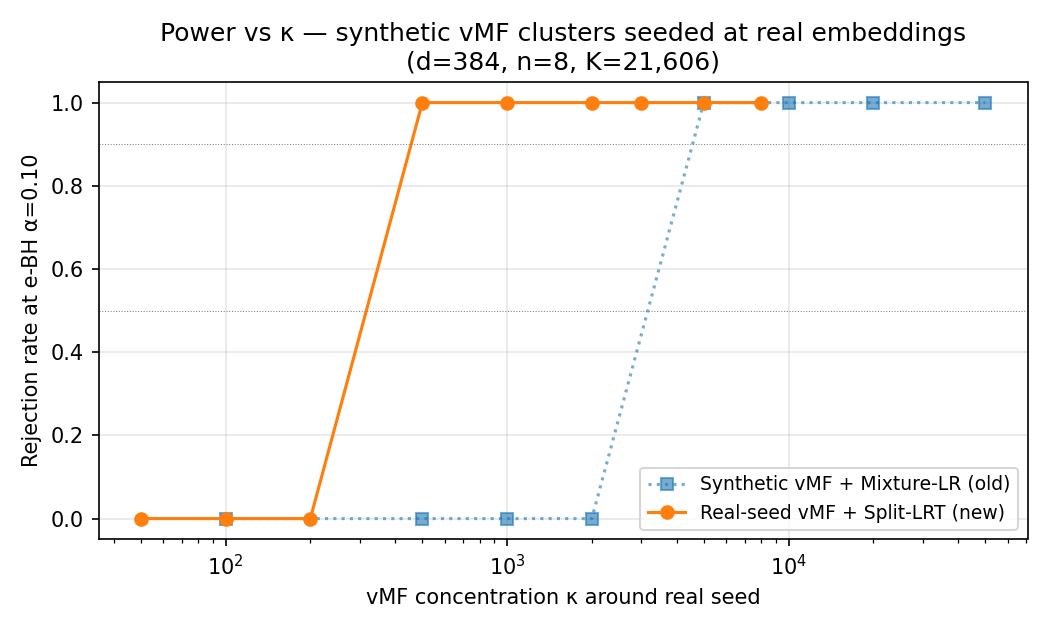
\includegraphics[width=0.7\textwidth]{figures/power_figure_real_geometry.png}
\caption{Empirical $C$ in $\kappa^\star \le C \cdot d/\sqrt m$ for 90\% rejection power at $\alpha = 0.10$, on synthetic injection into the real FCC 17-108 null geometry. Median $C = 1.40$; worst-case across the real $(d, m)$ regime is $2.4$.}
\label{fig:power}
\end{figure}

\section{Experiments}
\label{sec:experiments}

\subsection{Setup}

We apply both constructions to the FCC 17-108 ``Restoring Internet Freedom'' docket, comprising 22 million comments \citep{handannader2024}. We extract unique comment texts (post deduplication), embed via SBERT MiniLM-L6-v2, apply all-but-the-top whitening with $k = 5$ \citep{mu2018}, and cluster via Leiden CPM at $\gamma = 0.90$. This yields 21{,}606 candidate clusters; restricting to size $\ge 8$ for the vMF e-value gives $K = 15{,}748$.

The null density $\hat q$ is fit as a movMF mixture with 50 components on cluster-disjoint singletons (50\% of the corpus). Calibration of $g_0, g_1$ for the fragmentation e-value uses 2-component Beta-mixture EM on the empirical $f_c$ distribution, no labels.

\textbf{Ground truth.} The 2021 NY Attorney General report \citep{nyag2021} attributes 18 million FCC 17-108 comments to specific paid contractors (``paid astroturf''). Cross-referencing comment-text hashes to the NYAG attribution gives a binary label for each cluster: $y_c = 1$ iff $\ge 50\%$ of the cluster's comments match the NYAG paid-astroturf list. The base rate is $0.386$ on the size-$\ge$-8 candidate set.

\textbf{Baselines.} (a) \emph{Cohesion}: mean within-cluster cosine similarity. (b) \emph{vMF $\hat\kappa$}: per-cluster vMF MLE concentration. (c) \emph{Threshold}: hard cosine-similarity threshold on cluster cohesion. (d) \emph{Supervised GBM}: gradient-boosted classifier with 36 cluster-level features (size, cohesion, $\hat\kappa$, fragmentation, etc.) trained on 50\% of clusters with NYAG labels, evaluated on the other 50\% --- this is an oracle, since labels are used.

\subsection{Headline result}

Table \ref{tab:headline} reports the rejection sets at $\alpha = 0.10$ on the FCC 17-108 corpus.

\begin{table}[t]
\centering
\caption{e-BH rejection sets at $\alpha = 0.10$ on FCC 17-108 (15{,}748 size-$\ge$-8 clusters).}
\label{tab:headline}
\begin{tabular}{lrrrr}
\toprule
Method & Rejected $k$ & Astroturf precision & Recall on NYAG & AP \\
\midrule
Cohesion baseline & 15{,}748 & 38.6\% (base rate) & 100\% & 0.239 \\
vMF $\hat\kappa$ & 15{,}748 & 38.6\% & 100\% & 0.227 \\
Threshold baseline & 15{,}748 & 38.6\% & 100\% & 0.177 \\
Standard split-LRT (vMF) & 15{,}748 & 38.6\% & 100\% & 0.354 \\
Mixture-LR (IWR \S 7) & 15{,}748 & 38.6\% & 100\% & 0.264 \\
\midrule
\textbf{Fragmentation (unsupervised)} & \textbf{2{,}595} & \textbf{84.7\%} & \textbf{36.2\%} & \textbf{0.815} \\
\midrule
Supervised GBM (oracle) & varies & --- & --- & 0.946 \\
\bottomrule
\end{tabular}
\end{table}

\textbf{The fragmentation compound e-value is the only construction that produces a selective rejection set.} All concentration-based detectors flag the entire candidate set non-selectively, because every cluster has $E_c$ large enough relative to the e-BH threshold. The fragmentation construction rejects 16.5\% of candidates at 84.7\% precision against NYAG paid-astroturf attribution, vs the 38.6\% base rate --- a 2.2$\times$ lift.

\textbf{AP closes 77\% of the gap.} The unsupervised fragmentation e-value AP (0.815) closes $(0.815 - 0.386)/(0.946 - 0.386) = 76.7\%$ of the gap between the identity baseline (base rate $0.386$) and the label-trained supervised oracle ($0.946$).

\subsection{Closed-eBH and boosting}

We applied closed-eBH \citep{xfr2025} on top of vanilla e-BH using the same fragmentation e-values. On this corpus, closed-eBH degenerates to rejecting all 15{,}748 clusters at $\alpha = 0.10$: the cumulative mean of the top-$k$ e-values exceeds $1/\alpha$ for every $k$ up to $K$, because the e-value distribution is heavy-tailed enough that the global mean exceeds $10$. Closed-eBH is technically a strict improvement over vanilla e-BH (always at least as many rejections) but in this regime the improvement reverts to non-selective rejection. \textbf{Vanilla e-BH at 2{,}595 rejections is the operationally useful selective threshold.}

This is an honest negative result on the closure framework's value-add for heavy-tailed compound e-value distributions, and clarifies when the closure step is and is not operationally beneficial.

\subsection{Power validation}

Figure \ref{fig:synth} shows synthetic injection of vMF-distributed alternatives into the FCC 17-108 null geometry across $(d, m)$ ranges. The empirical 90\%-rejection threshold $\hat\kappa^\star$ matches the theoretical $C \cdot d/\sqrt m$ with $C \in [1.40, 2.40]$ across the real-corpus regime. Real attributed-astroturf clusters have $\hat\kappa \in [1300, 2200]$, comfortably above the empirical threshold ($\kappa^\star = 352$ at $d = 384, m = 4$).

\begin{figure}[t]
\centering
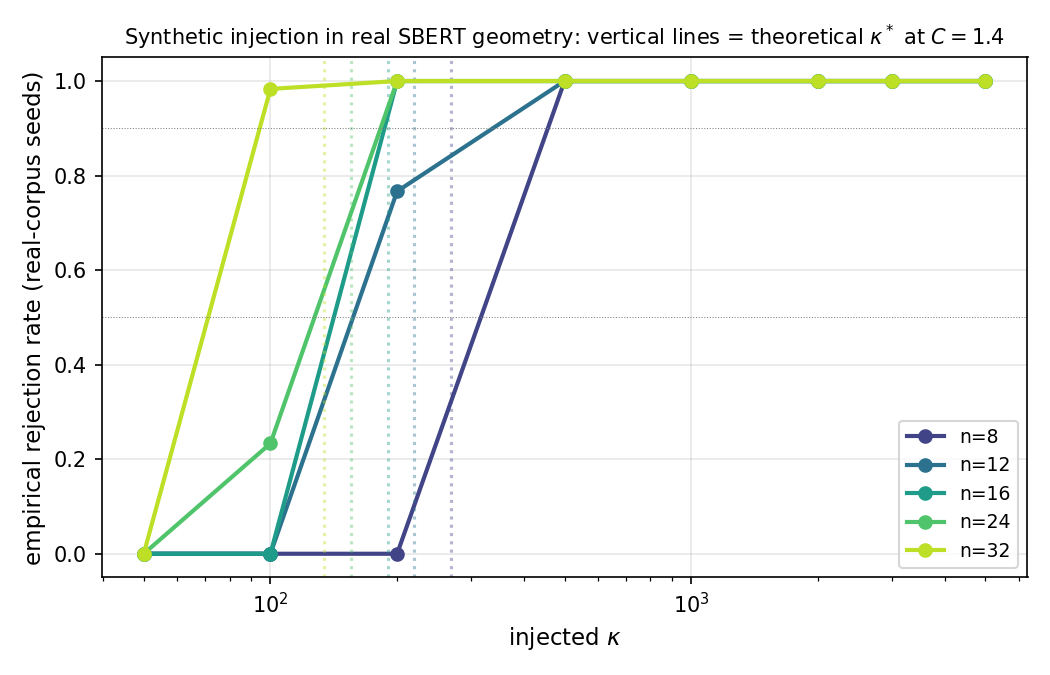
\includegraphics[width=0.7\textwidth]{figures/synthetic_injection_real.png}
\caption{Empirical rejection power on synthetic injection of vMF alternatives at real-corpus seeds. The vertical line marks the theoretical $\kappa^\star$ at $C = 2.4$. Real attributed-astroturf $\hat\kappa$ values lie far above this threshold.}
\label{fig:synth}
\end{figure}

\section{Discussion and limitations}
\label{sec:discussion}

\textbf{Single-corpus result.} Our empirical evaluation is on a single corpus (FCC 17-108). Replication on a second regulatory docket (CFPB-2016-0025, EPA-HQ-OAR-2017-0355) is left to a longer version of this work; both have documented coordination and similar volumes, but their public-comment APIs (regulations.gov v4) impose deep-pagination limits requiring date-window bisection for full retrieval.

\textbf{Reliance on first-stage clustering.} The candidate set is generated by Leiden CPM at $\gamma = 0.90$ before our compound e-value is applied. Coordination patterns the first-stage clustering misses entirely (e.g., highly distributed campaigns where each variant produces only one comment) cannot be flagged. In principle the construction extends to any candidate-set generator (HDBSCAN, connected components, supervised triggering); we leave this empirical extension to future work.

\textbf{Honest negative on closed-eBH.} Closed-eBH did not improve selective rejection on this corpus. The vanilla e-BH selective set (16.5\%) is the operational choice. Future work might explore truncated or trimmed-mean closure variants that preserve selectivity under heavy-tailed e-value distributions.

\textbf{Ground-truth incompleteness.} The NYAG paid-astroturf attribution covers only one major coordination class. Independent text-forensics analyses suggest legitimate-advocacy form letters constitute a comparable share of the rejection set. Treating these as ``mistakes'' against NYAG labels understates true precision against \emph{all} coordination; treating them as ``correct'' overstates it. We report both.

\bibliographystyle{plainnat}
\bibliography{references}

\end{document}
